

\documentclass[9pt]{beamer}
\mode<presentation>
\linespread{1.5}

\usetheme{Madrid}
%\usetheme {CambridgeUS}%{Goettingen}%{Berkeley}%{Montpellier}%{Antibes}%{Dresden}%{Madrid}%{Dresden}%{Darmstadt}%{Warsaw}%{Pittsburgh}
\usefonttheme{{structuresmallcapsserif}}%{structureitalicserif}%{structurebold}%{structuresmallcapsserif}%{professionalfonts}
%\useoutertheme[subsection=false]{smoothbars}
\usepackage[english]{babel}
%\usepackage[latin1]{inputenc}
\usepackage{hyperref}
%\usecolortheme{beaver}
%\usecolortheme{crane}

%\setbeamercovered{transparent}
%\newcommand{\semitransp}[2][35]{\color{fg!#1}#2}

\usepackage{latexsym}
\usepackage{amsmath}
\usepackage{times}
%\usepackage{MinionPro}
\usepackage{hyperref}
\usepackage{tikz}
\usepackage{verbatim}
\usepackage{natbib}
\usepackage{color, colortbl}
\usepackage{appendix}
\usepackage{ulem}
\usepackage{amsmath,amsthm}

\usetikzlibrary{arrows,shapes}


\newtheorem{proposition}{Proposition}[section]
%\newtheorem{definition}{Definition}[section]
\newtheorem{assumption}{Assumption}[section]
\newtheorem{conjecture}{Conjecture}[section]
\newtheorem*{observation}{Observation}


\definecolor{Gray}{gray}{0.9}


\pgfdeclarelayer{background}
\pgfsetlayers{background,main}

\tikzstyle{vertex}=[circle,fill=black!25,minimum size=12pt,inner sep=0pt]
\tikzstyle{selected vertex} = [vertex, fill=red!24]
\tikzstyle{unknown vertex} = [vertex, fill=black]
\tikzstyle{edge} = [draw,thick,-]
\tikzstyle{weight} = [font=\small]
\tikzstyle{selected edge} = [draw,line width=5pt,-,red!50]
\tikzstyle{ignored edge} = [draw,line width=5pt,-,black!20]







\title{Coordination in Social Networks}
\author{Chun-Ting Chen}


\begin{document}

\maketitle


\section{Introduction}
\subsection{Motivation}


\frame{
  \frametitle{Motivation}

\begin{itemize}[<+->]
\item An exogenous network models restricted information in collective action. 
\begin{itemize}
\item ~[Chwe] models incomplete information.
\item ~[Wolitzky] models network-monitoring.
\end{itemize}


\item This paper provides a partial folk theorem with incomplete information and network-monitoring.
\begin{itemize}
\item Will people act collectively in networks \textbf{eventually}? 
\end{itemize}

\end{itemize}

}


\frame{
  \frametitle{Motivation}

\begin{itemize}[<+->]
\item ~[Chwe]: one-shot collective action (in terms of revolution).
\begin{itemize}
\item Players of two types (\textbf{Rebel},\textbf{Inert}). They can \textbf{observe own/neighbor's type}. 
\item Rebel's pay-off contingent on global type distribution.

\end{itemize}

\item ~[Chwe]'s result: the ex-post efficient outcome ``guaranteed'' by complete network.

\end{itemize}

}


\frame{
  \frametitle{What this paper does?}

\begin{itemize}[<+->]
\item \alert{Model}: repeated collective actions (in terms of protest).
\begin{itemize}
\item Types are fixed over time.
\item Players can observe \textbf{own/neighbors' types}.
\item Players can observe \textbf{own/neighbors' actions}.
\end{itemize}
\item \alert{Goal}: looking for an equilibrium, in which the global type distribution becomes commonly known in finite time.
\item \alert{Result}: such equilibrium can be constructed under some assumptions.
\end{itemize}

}


\subsection{Literature Review}
\frame{
  \frametitle{Related Literature}

  \begin{itemize}
  \item Collective action.
  \begin{itemize}
  \item One strand: [Chwe 2000], [Lohmann, 1993,1994], etc 
  \item \textbf{This paper adds network-monitoring}
  \end{itemize}
\pause
  \item Repeated game in networks.
  \begin{itemize}
  \item One strand: [Wolitzky 2013] 
  \item \textbf{This paper adds incomplete information}
  \end{itemize}
 
\end{itemize}

}









\section{Model}
\subsection{Static Game}







\frame{
  \frametitle{Model}

Network
  \begin{itemize}
\item $n$ players; $N=\{1,...,n\}$ is the set of players. 
  \item $G_i$ is $i$'s neighborhood; $G_i$ is a subset of $N$ such that $i\in G_i$.
  
  \item $G=\{G_i\}_i$ is the network.
 
  \end{itemize}



\begin{assumption}
$G$ is fixed (not random), finite, connected, commonly known, and undirected.
\end{assumption}

 

}

\frame{
  \frametitle{Model}

Static $k$-threshold game [Chwe 2000]
  \begin{itemize}
    
    \item $1\leq k \leq n$
    \pause
 \item $\theta_i\in \Theta_i=\{Rebel,Inert\}$: $i$'s type 
  \item $\theta\in \Theta=\times_{i\in N}\Theta_i$: type profile 
  \item $\pi\in \Delta \Theta$: the prior  \pause
  \item $A_{Rebel}=\{\textbf{revolt},\textbf{stay}\}$; $A_{Inert}=\{\textbf{stay}\}$

 

  \end{itemize}


}

\begin{frame}[label=static_game]
  \frametitle{Model}
Static $k$-threshold game [Chwe 2000]: \hyperlink{alt_static_game}{\beamergotobutton{Or}}

  \begin{itemize}
  \item Static game payoff for Rebel $i$: $u_{Rebel_i}(a_{Rebel_i},a_{-\theta_i})$

\end{itemize}
  \begin{table}[h]
\begin{tabular}{llll}
$u_{Rebel_i}(a_{Rebel_i},a_{-\theta_i})$ & $=$ & 1 & if $a_{Rebel_i}=\textbf{revolt}$ and $\#\{j:a_{\theta_j}=\textbf{revolt}\}\geq k$ \\
$u_{Rebel_i}(a_{Rebel_i},a_{-\theta_i})$ & $=$ & -1 & if $a_{Rebel_i}=\textbf{revolt}$ and $\#\{j:a_{\theta_j}=\textbf{revolt}\}< k$ \pause \\
\\
$u_{Rebel_i}(a_{Rebel_i},a_{-\theta_i})$ & $=$ & 0 & if $a_{Rebel_i}=\textbf{stay}$ \pause \\
\end{tabular}

\end{table}

\begin{assumption}

Players perfectly observe their neighbors' types.

\end{assumption}

 \begin{itemize}
 \item \textit{Remark}: \textbf{stay} is a safe arm; \textbf{revolt} is a risky arm.
 \end{itemize}

\end{frame}


\begin{frame}
  \frametitle{Model}
Static $k$-threshold game [Chwe 2000]-example

\begin{itemize}
\item $n=3$ and $k=3$
\end{itemize}

\begin{center}
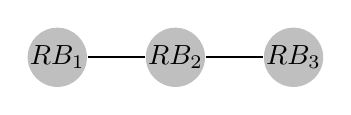
\begin{tikzpicture}[scale=1.5]
    % Draw a 7,11 network
    % First we draw the vertices
    \foreach \pos/\name in {{(1,0)/RB_1}, {(2,0)/RB_2}, {(3,0)/RB_3}}
        \node[vertex] (\name) at \pos {$\name$};
    % Connect vertices with edges 
    \foreach \source/ \dest in {RB_1/RB_2, RB_2/RB_3}
        \path[edge] (\source) -- (\dest) ;
        
\end{tikzpicture}
\end{center}


\begin{itemize}
\item For some $\pi$, this network does not sustain ex-post efficient outcome.
\end{itemize}

\end{frame}




\subsection{Repeated Game}


\begin{frame}
  \frametitle{Model}
Repeated $k$-threshold game: time line
  \begin{itemize}

  \item Nature choose $\theta$ initially according to $\pi$.

  \item Types are then fixed over time.

  \item Players play the static $k$-threshold game infinitely repeatedly.


  \end{itemize}

\begin{assumption}
\begin{itemize}
    \item Players perfectly observe their neighbors' types.
\item Players perfectly observe their neighbors' actions. 
  \item $\pi$ has full support

\item Common $\delta$. 
\item Static pay-off could be observable, noisy or hidden.
\end{itemize}

\end{assumption}

\end{frame}


\begin{frame}
  \frametitle{Model}

Look for
\begin{itemize}
\item An equilibrium, the ex-post efficient outcome repeats after some finite time $T$ in the path.
\end{itemize}

\end{frame}






\begin{frame}
  \frametitle{Model}

Notations:
\begin{itemize}
\item $[Rebels](\theta)=\{j:\theta_j=Rebel\}$ for all $\theta\in \Theta$. 
\item $\# [Rebels](\theta)$: number of Rebels given $\theta$ \pause
\item $\theta_{G_i}$: $i$'s private information about the state. ($\theta_{G_i}\in \Theta_{G_i}=\prod_{j\in G_i}\Theta_j$)
\item $h^{m}_{G_i}$: the history observed by $i$ up to period $m$. ($h^{m}_{G_i}\in H^{m}_{G_i}=\prod^m_{s=1}\prod_{j\in G_i}A_{\theta_j}$)
\item $h$: an infinite sequence of players' actions. ($h\in H=\prod^{\infty}_{s=1}\prod_{j\in N}A_{\theta_j}$) \pause 
\item $\tau_i:\Theta_{G_i}\times \bigcup^{\infty}_{0} H^{m}_{G_i} \rightarrow A_{\theta_i}$, $i$'s strategy.
\item $\tau=(\tau_1,...,\tau_i,...,\tau_n)$: a strategy profile. \pause
\item $\beta^{\pi,\tau}_i(\theta|h^{m}_{G_i})$: $i$'s belief for a $\theta$ at period $m$ given $\tau$.

 
\end{itemize}

\end{frame}

\begin{frame}
  \frametitle{APEX}
Notations:
\begin{itemize}
\item $h^{\tau}_{\theta}$ : a history generated by $\tau$ given $\theta$.
\item Call $h^{\tau}_{\theta}$ a $\tau_{\theta}$-path.
\item Call $\{h^{\tau}_{\theta}\}_{\theta\in \Theta}$ the $\tau$-path
\end{itemize}


\begin{definition}
The $\tau$-path is \textbf{approaching ex-post efficient} (\textit{APEX}) $\Leftrightarrow$ 
\[\text{$\forall\theta$,  there is a finite time $T^{\theta}$}\] 
such that the actions after $T^{\theta}$ in $\tau_{\theta}$ repeats the static ex-post efficient outcome.
\end{definition}
 


\end{frame}



\begin{frame}
  \frametitle{APEX}


\begin{definition}[weak APEX equilibrium]
A weak sequential equilibrium $(\tau^{*},\beta^{*})$ is APEX $\Leftrightarrow$ $\tau^{*}$-path is APEX, and $\beta^{*}$ is the belief system consistent with $\tau^{*}$.
\end{definition}
\pause
\begin{definition}[APEX equilibrium]
A sequential equilibrium $(\tau^{*},\beta^{*})$ is APEX $\Leftrightarrow$ $(\tau^{*},\beta^{*})$ is a weak APEX equilibrium and $\beta^{*}$ is fully consistent with $\tau^{*}$[Krep and Wilson 1982].
\end{definition}

\end{frame}




\frame{
  \frametitle{APEX for $k=n$}

\begin{itemize}
\item $k=n$: For all networks, an APEX equilibrium can be found whenever $\delta$ is sufficiently high.

\end{itemize}


}


\begin{frame}
  \frametitle{APEX-example for $k=n$}

\alert{\textbf{If pay-off is observable}}, for $k=n=3$:
  \begin{center}
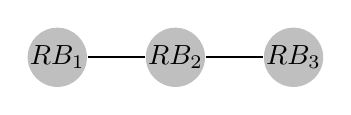
\begin{tikzpicture}[scale=1.5]
    % Draw a 7,11 network
    % First we draw the vertices
    \foreach \pos/\name in {{(1,0)/RB_1}, {(2,0)/RB_2}, {(3,0)/RB_3}}
        \node[vertex] (\name) at \pos {$\name$};
    % Connect vertices with edges 
    \foreach \source/ \dest in {RB_1/RB_2, RB_2/RB_3}
        \path[edge] (\source) -- (\dest) ;
        
\end{tikzpicture}
\end{center}

\begin{itemize}[<+->]
\item All Rebels play \textbf{revolt} in the first period $\Rightarrow$ then state will be revealed.
\end{itemize}

  
\end{frame}


\begin{frame}
  \frametitle{APEX-example for $k=n$}

\alert{\textbf{If pay-off is hidden or noisy}}, for $k=n=3$:

\begin{enumerate} [<+->]
\item   
\begin{center}
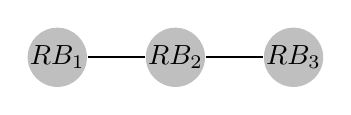
\begin{tikzpicture}[scale=1.5]
    % Draw a 7,11 network
    % First we draw the vertices
    \foreach \pos/\name in {{(1,0)/RB_1}, {(2,0)/RB_2}, {(3,0)/RB_3}}
        \node[vertex] (\name) at \pos {$\name$};
    % Connect vertices with edges 
    \foreach \source/ \dest in {RB_1/RB_2, RB_2/RB_3}
        \path[edge] (\source) -- (\dest) ;
        
\end{tikzpicture}
\end{center}

\begin{itemize}
\item Rebel 2 chooses $\textbf{revolt}$ at the first period $\Rightarrow$ the state can be revealed.

\end{itemize}
\item
\begin{center}
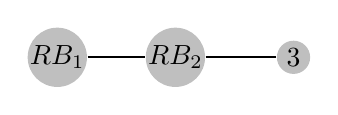
\begin{tikzpicture}[scale=1.5]
    % Draw a 7,11 network
    % First we draw the vertices
    \foreach \pos/\name in {{(1,0)/RB_1}, {(2,0)/RB_2}, {(3,0)/3}}
        \node[vertex] (\name) at \pos {$\name$};
    % Connect vertices with edges 
    \foreach \source/ \dest in {RB_1/RB_2, RB_2/3}
        \path[edge] (\source) -- (\dest) ;
        
\end{tikzpicture}
\end{center}

\begin{itemize}
\item Rebel 2 chooses $\textbf{stay}$ at the first period $\Rightarrow$ the state can be revealed.

\end{itemize}
\end{enumerate}


  
\end{frame}






\frame{
  \frametitle{APEX for $k<n$}

\begin{itemize}
\item $k<n$: with additional assumptions,
\begin{itemize}
\item acyclic networks (tree networks): a weak APEX equilibrium can be found when $\delta$ is high enough.
\item cyclic networks: open question.
\end{itemize}
\end{itemize}

}


\begin{frame}
  \frametitle{Acyclic network: definition}


\begin{definition}[Path in a network]
A \textbf{path} from node $i$ to node $j$ is a sequence of nodes \[\{i,m_1,m_2,...,m_n,j\} \text{ without repetition }\] such that $i\in G_{m_1},m_1\in G_{m_2},...,m_n\in G_j$. 
\end{definition}  

\begin{definition}[Acyclic network (Tree)]
A network is \textbf{acyclic} $\Leftrightarrow$ the path from node $i$ to node $j$ is unique for all nodes $i,j$. 
\end{definition}  

\end{frame}


\begin{frame}
  \frametitle{APEX-example for $k<n$}

\alert{\textbf{If pay-off is observable}}, for $k=3$ and $n=4$:
  \begin{center}
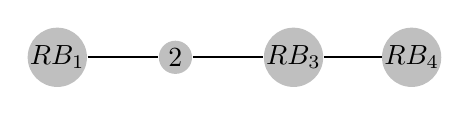
\begin{tikzpicture}[scale=1.5]
    % Draw a 7,11 network
    % First we draw the vertices
    \foreach \pos/\name in {{(1,0)/RB_1}, {(2,0)/2}, {(3,0)/RB_3}, {(4,0)/RB_4}}
        \node[vertex] (\name) at \pos {$\name$};
    % Connect vertices with edges 
    \foreach \source/ \dest in {RB_1/2, 2/RB_3, RB_3/RB_4}
        \path[edge] (\source) -- (\dest) ;
        
\end{tikzpicture}
\end{center}

\begin{itemize}[<+->]
\item All Rebels play \textbf{revolt} in the first period $\Rightarrow$ then state will be revealed.
\end{itemize}

  
\end{frame}

\begin{frame}
  \frametitle{APEX-example for $k<n$}

\alert{\textbf{If pay-off is hidden or noisy}}, for $k=3$ and $n=4$:
  \begin{center}
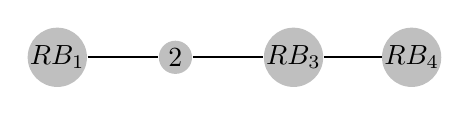
\begin{tikzpicture}[scale=1.5]
    % Draw a 7,11 network
    % First we draw the vertices
    \foreach \pos/\name in {{(1,0)/RB_1}, {(2,0)/2}, {(3,0)/RB_3}, {(4,0)/RB_4}}
        \node[vertex] (\name) at \pos {$\name$};
    % Connect vertices with edges 
    \foreach \source/ \dest in {RB_1/2, 2/RB_3, RB_3/RB_4}
        \path[edge] (\source) -- (\dest) ;
        
\end{tikzpicture}
\end{center}

\begin{itemize}[<+->]
\item An APEX equilibrium does not exist.
\end{itemize}

  
\end{frame}




\begin{frame}
  \frametitle{Strong connectedness}


\begin{definition}
$\theta$ has \textbf{Strong connectedness}$\Leftrightarrow$ for every pair of Rebels, there is a path consisting of Rebels to connect them.
\end{definition}  

\begin{definition}
$\pi$ has \textbf{full support on strong connectedness}$\Leftrightarrow$ 
\[\text{$\pi(\theta)>0$ if and only if $\theta$ has strong connectedness.}\]
\end{definition}  
\begin{itemize}
\item I.e. Commonly certainty of strong connectedness.
\end{itemize}
\pause
\begin{assumption}
$\pi$ has \textbf{full support on strong connectedness}.
\end{assumption}

\end{frame}


\begin{frame}
  \frametitle{APEX-example for $k<n$}

\alert{\textbf{If pay-off is hidden or noisy}}, for $k=3$ and $n=4$ with strong connectedness:
  \begin{center}
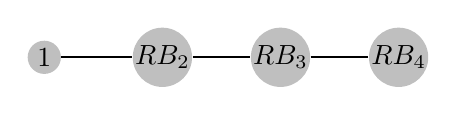
\begin{tikzpicture}[scale=1.5]
    % Draw a 7,11 network
    % First we draw the vertices
    \foreach \pos/\name in {{(1,0)/1}, {(2,0)/RB_2}, {(3,0)/RB_3}, {(4,0)/RB_4}}
        \node[vertex] (\name) at \pos {$\name$};
    % Connect vertices with edges 
    \foreach \source/ \dest in {1/RB_2, RB_2/RB_3, RB_3/RB_4}
        \path[edge] (\source) -- (\dest) ;
        
\end{tikzpicture}
\end{center}

\begin{itemize}[<+->]
\item An APEX equilibrium exists---same idea: Rebel 3 play a ``\textit{coordination message}'' $\Rightarrow$ state can be revealed.
\item Later, I generalize the case of $k<n$ for acyclic networks. 
\end{itemize}

  
\end{frame}


\section{Equilibrium construction}
\subsection{Equilibrium construction}

\frame{
  \frametitle{Case of $k<n$}
\framesubtitle{Equilibrium construction}


Outline: 

\begin{enumerate}
\item Communication by actions \pause
\item Communication in the equilibrium
\begin{enumerate}
\item Communication protocol
\item In-the-path belief 
\item Off-path belief
\item Sketch of proof
\end{enumerate}

\end{enumerate}

}




\begin{frame}
  \frametitle{Communication by actions}
\framesubtitle{Main idea}

Ex. for $n=5$ network:
  \begin{center}
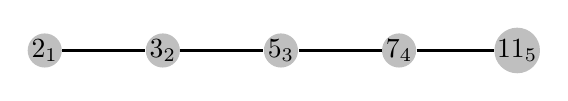
\begin{tikzpicture}[scale=1.5]
    % Draw a 7,11 network
    % First we draw the vertices
    \foreach \pos/\name in {{(1,0)/2_1}, {(2,0)/3_2}, {(3,0)/5_3}, {(4,0)/7_4}, {(5,0)/11_5}}
        \node[vertex] (\name) at \pos {$\name$};
    % Connect vertices with edges 
    \foreach \source/ \dest in {2_1/3_2, 3_2/5_3, 5_3/7_4, 7_4/11_5}
        \path[edge] (\source) -- (\dest) ;
        
\end{tikzpicture}
\end{center}

\begin{itemize}[<+->]
\item First step: index each node a distinguish prime number.
\item This indexation is commonly known.
\end{itemize}

\end{frame}

\begin{frame}
  \frametitle{Communication by actions}
\framesubtitle{Main idea-conti}

Ex. for $k=4$, $n=5$ with strong connectedness:
  \begin{center}
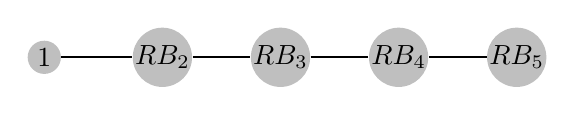
\begin{tikzpicture}[scale=1.5]
    % Draw a 7,11 network
    % First we draw the vertices
    \foreach \pos/\name in {{(1,0)/1}, {(2,0)/RB_2}, {(3,0)/RB_3}, {(4,0)/RB_4}, {(5,0)/RB_5}}
        \node[vertex] (\name) at \pos {$\name$};
    % Connect vertices with edges 
    \foreach \source/ \dest in {1/RB_2, RB_2/RB_3, RB_3/RB_4, RB_4/RB_5}
        \path[edge] (\source) -- (\dest) ;
        
\end{tikzpicture}
\end{center}

\begin{itemize}[<+->]
\item Second step: build a communication protocol.
\item If the incentive issue is ignored, ideally,
\begin{table}[h]
\begin{tabular}{l l l l}
& \textit{Reporting period} & \textit{Coordination period} & ...\\
\hline
& 1,2,...,2310 & 2311,...,2421 & 2422,...\\
\hline
$RB_2$ & $\textbf{s},...,\textbf{s},\overbrace{\textbf{r},\textbf{s},...,\textbf{s}}^{2\times 3}$ & $\neg$ send ``coordination message''  & play \textbf{revolt afterwards}\\
$RB_3$ & $\textbf{s},...,\textbf{s},\overbrace{\textbf{r},\textbf{s},...,\textbf{s}}^{2\times 3\times 5}$ &  send ``coordination message'' & play \textbf{revolt afterwards}
\end{tabular}
\end{table}
\end{itemize}

\end{frame}






\begin{frame}
  \frametitle{Communication Phases}


Phases 
\begin{enumerate}
\item<1-> \textbf{RP} (Reporting period): revealing the information about $\theta$. 
\item<1-> \textbf{CD} (Coordination period): coordinating the future actions.
\item<2-> RP and CD alternate finitely.
\[\underbrace{\langle RP \rangle \langle CD \rangle}_{\onslide<3>{\textbf{{block}}}}...\]
\item<3> Call a complete two phases, $\langle RP \rangle \langle CD \rangle$, a \textbf{block}. 
\end{enumerate}







\end{frame}








\begin{frame}


\frametitle{Coordination period and messages}


In coordination period, 
\begin{itemize}
\item ``three'' messages coordinate actions

\begin{table}[h]
\begin{tabular}{l l}
Messages & Continuation actions\\
\hline
\textbf{message to {revolt}}& play \textbf{revolt} afterward\\
\textbf{message to {stay}} & play \textbf{stay} afterward\\
Other messages &  continue to next block 
\end{tabular}
\end{table}

\end{itemize}



\end{frame}







\begin{frame}[label=protocol_grim_trigger]
\frametitle{Coordination period and messages}



\begin{itemize}
\item Communication either stops or continues after a CD.
\begin{enumerate}
\item {Stopping}: If \textbf{Message to stay} or \textbf{Message to revolt} is sent \ $\Rightarrow$ all Rebels coordinate to play same actions. 
\item {Continuing}: Otherwise, go to the next block.
\end{enumerate}

\end{itemize}

\pause
\begin{lemma}
Before a Rebel knows $\#[Rebels](\theta)< k$ or $\#[Rebels](\theta)\geq k$ , he will not send \textbf{Message to stay} or \textbf{Message to revolt} if $\delta$ is high enough.
\end{lemma}
\begin{itemize}
\item a ``grim trigger''.
\end{itemize}
\hyperlink{CD_to_RP}{\beamergotobutton{Comment}}
\end{frame}










\begin{frame}
\frametitle{Reporting period and messages}



\begin{itemize}
\item $RP^t$: the reporting period at $t$ block

\item $\langle RP^t \rangle$: the reporting message
\begin{table}[h]
\begin{tabular}{l l l}
\alert{Costly message} & $\neg\langle \textbf{stay} \rangle$ & $\textbf{s},...,\textbf{s},{\textbf{r},\textbf{s},...,\textbf{s}}$ \\
\hline
\alert{Not costly message} & $\langle \textbf{stay} \rangle$ & $\textbf{s},...,\textbf{s},\textbf{s},\textbf{s},...,\textbf{s}$  \\

\end{tabular}
\end{table}

\pause
\item Gives incentive to play costly message.
\begin{enumerate}
\item {Costly message}+\textbf{message to revolt}: coordination to \textbf{revolt}

\item Otherwise, no coordination to \textbf{revolt}


\end{enumerate}

\pause

\item How much cost should a Rebel take? --- Characterization in the next slides.

\end{itemize}








\end{frame}






\begin{frame}
   \frametitle{Information Hierarchy}


\textbf{Information Hierarchy}
\begin{itemize}
\item {Characterizing Rebels' incentives in playing costly messages}\hyperlink{alt_IH}{\beamergotobutton{other reason}}
\end{itemize}

Ex: 
\begin{center}
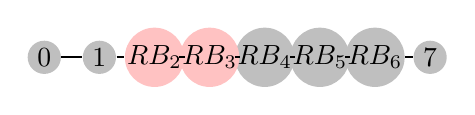
\begin{tikzpicture}[scale=0.7]
    % Draw a 7,11 network
    % First we draw the vertices
    \foreach \pos/\name in {{(0,1)/1},{(6,1)/7},{(-1,1)/0}, {(3,1)/RB_4}, {(4,1)/RB_5}, {(5,1)/RB_6}}
        \node[vertex] (\name) at \pos {$\name$};
        
    \foreach \pos/\name in {{(1,1)/RB_2}, {(2,1)/RB_3}}
    \node[selected vertex] (\name) at \pos {$\name$};
    
    % Connect vertices with edges 
    \foreach \source/ \dest in {1/RB_2,RB_2/RB_3, RB_3/RB_4, RB_4/RB_5, RB_5/RB_6,RB_6/7,0/1}
        \path[edge] (\source) -- (\dest) ;
        
\end{tikzpicture}
\end{center}

\pause
\begin{itemize}
\item \textbf{Rebel 2 has less incentive}: Rebel 2's information can be reported by Rebel 3 to Rebel 4.
\end{itemize}



\end{frame}
















\begin{frame}[label=IH]
  \frametitle{Information Hierarchy}

\textbf{Information Hierarchy}  

\onslide<1->{  
\begin{center}
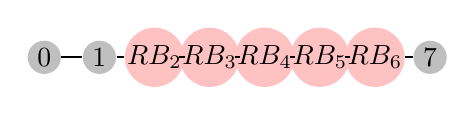
\begin{tikzpicture}[scale=0.7]
    % Draw a 7,11 network
    % First we draw the vertices
    \foreach \pos/\name in {{(0,1)/1},{(6,1)/7},{(-1,1)/0}}
        \node[vertex] (\name) at \pos {$\name$};
        
    \foreach \pos/\name in {{(1,1)/RB_2}, {(2,1)/RB_3}, {(3,1)/RB_4}, {(4,1)/RB_5}, {(5,1)/RB_6}}
    \node[selected vertex] (\name) at \pos {$\name$};
    
    % Connect vertices with edges 
    \foreach \source/ \dest in {1/RB_2,RB_2/RB_3, RB_3/RB_4, RB_4/RB_5, RB_5/RB_6,RB_6/7,0/1}
        \path[edge] (\source) -- (\dest) ;
        
\end{tikzpicture}
\end{center}
}

\onslide<2->{
\begin{center}
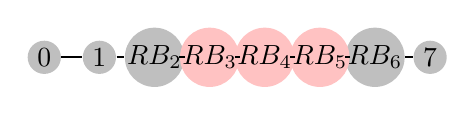
\begin{tikzpicture}[scale=0.7]
    % Draw a 7,11 network
    % First we draw the vertices
    \foreach \pos/\name in {{(0,1)/1},{(6,1)/7},{(1,1)/RB_2},{(5,1)/RB_6},{(-1,1)/0}}
        \node[vertex] (\name) at \pos {$\name$};
        
    \foreach \pos/\name in {{(2,1)/RB_3}, {(3,1)/RB_4}, {(4,1)/RB_5}}
    \node[selected vertex] (\name) at \pos {$\name$};
    
    % Connect vertices with edges 
    \foreach \source/ \dest in {1/RB_2,RB_2/RB_3, RB_3/RB_4, RB_4/RB_5, RB_5/RB_6,RB_6/7,0/1}
        \path[edge] (\source) -- (\dest) ;
        
\end{tikzpicture}
\end{center}
}

\onslide<3>{
\begin{center}
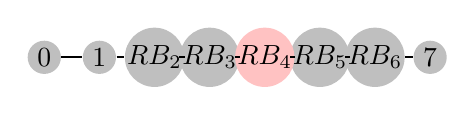
\begin{tikzpicture}[scale=0.7]
    % Draw a 7,11 network
    % First we draw the vertices
    \foreach \pos/\name in {{(0,1)/1},{(6,1)/7},{(1,1)/RB_2},{(5,1)/RB_6},{(2,1)/RB_3}, {(4,1)/RB_5},{(-1,1)/0}}
        \node[vertex] (\name) at \pos {$\name$};
        
    \foreach \pos/\name in { {(3,1)/RB_4}}
    \node[selected vertex] (\name) at \pos {$\name$};
    
    % Connect vertices with edges 
    \foreach \source/ \dest in {1/RB_2,RB_2/RB_3, RB_3/RB_4, RB_4/RB_5, RB_5/RB_6,RB_6/7,0/1}
        \path[edge] (\source) -- (\dest) ;
        
\end{tikzpicture}
\end{center}
}



\begin{enumerate}
\item \onslide<1-> At $\alert{0}$-block, let $\alert{R^0}=\{2,3,4,5,6\}$
\item \onslide<2-> At $\alert{1}$-block, let $\alert{R^1}=\{\invisible{2,}3,4,5\invisible{,6}\}$
\item \onslide<3> At $\alert{2}$-block, let $\alert{R^2}=\{\invisible{2,}\invisible{3,}4\invisible{,5}\invisible{,6}\}$
\end{enumerate}

\hyperlink{IH_details}{\beamergotobutton{details}}

\end{frame}





\begin{frame}
  \frametitle{Information Hierarchy}

The Rebels known by $i$ after $t$-block: $I^t_i$.
\begin{theorem}
\label{lemma_empty}
Given $\theta$, if
\begin{enumerate}
\item the network is acyclic
\item the state has strong connectedness
\end{enumerate}
$\Rightarrow$ $\exists t^{\theta}$ and $\exists i\in R^{t^{\theta}}$ such that $I^{t^{\theta}}_i \supset [Rebels](\theta) $.
\end{theorem} 

\bigskip

Thus, ideally, APEX can be attained by
\begin{itemize}
\item At $t$ block

\begin{table}[h]
\begin{tabular}{l l l l}
$R^t$ Rebels & play & $\langle I^{t-1}_i\rangle$ & $\textbf{s},...,\textbf{s},\overbrace{\textbf{r},\textbf{s},...,\textbf{s}}^{\text{Multiplication of $I^{t-1}_i$ Rebels' prime numbers}}$ \\
\hline
non-$R^t$ Rebels & play & $\langle \textbf{stay} \rangle$ & $\textbf{s},...,\textbf{s},\textbf{s},\textbf{s},...,\textbf{s}$  \\

\end{tabular}
\end{table}
\pause
\item \alert{However, ``Pivotal Rebels'' will deviate}.

\end{itemize}
\end{frame}


\begin{frame}
  \frametitle{Information Hierarchy}

\framesubtitle{Pivotal players}

Relevant information: $\#[Rebels](\theta)\geq k$ or $\#[Rebels](\theta)<k$.

\begin{definition}[Pivotal player in $RP^t$]
$i$ is \textbf{pivotal} in $RP^t$
\[ \Leftrightarrow \]
$i\in R^t$ and $i$ {will} learn the relevant info {before} $I^{t-1}_i$ is reported {given} others' truthful reporting.
\end{definition}


\end{frame}

\begin{frame}[label=acyclic_diss]
  \frametitle{Information Hierarchy}
\framesubtitle{Pivotal players}



Ex. $k=5$,
\begin{center}
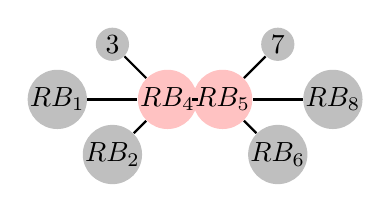
\begin{tikzpicture}[scale=0.7]
    % Draw a 7,11 network
    % First we draw the vertices
    \foreach \pos/\name in {{(1,2)/RB_1}, {(2,1)/RB_2}, {(2,3)/3}, {(5,1)/RB_6}, {(5,3)/7}, {(6,2)/RB_8}}
        \node[vertex] (\name) at \pos {$\name$};
    
    \foreach \pos/\name in {{(3,2)/RB_4}, {(4,2)/RB_5}}
    \node[selected vertex] (\name) at \pos {$\name$};
    
    % Connect vertices with edges 
    \foreach \source/ \dest in {RB_1/RB_4, RB_2/RB_4,3/RB_4,RB_4/RB_5, RB_5/RB_6, RB_5/7, RB_5/RB_8}
        \path[edge] (\source) -- (\dest) ;
        
\end{tikzpicture}
\end{center}
\begin{enumerate}
\item Rebel 4 and Rebel 5 are pivotal (\textbf{Free Rider problem})
\item They can manipulate their reporting to save costs.

\end{enumerate}


\hyperlink{cyclic_diss}{\beamergotobutton{Go to discussion}}
\end{frame}



\begin{frame}
  \frametitle{Information Hierarchy}

\framesubtitle{Pivotal players}


Ex. $k=6$, 
\begin{center}
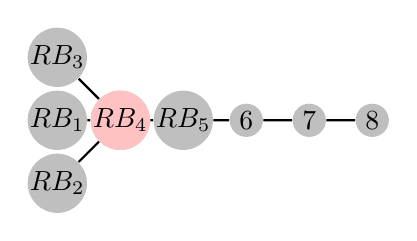
\begin{tikzpicture}[scale=0.8]
    % Draw a 7,11 network
    % First we draw the vertices
    \foreach \pos/\name in {{(2,2)/RB_1}, {(2,1)/RB_2}, {(2,3)/RB_3}, {(3,2)/RB_4}, {(4,2)/RB_5}, {(5,2)/6}, {(6,2)/7}, {(7,2)/8}}
        \node[vertex] (\name) at \pos {$\name$};
    
    \foreach \pos/\name in { {(3,2)/RB_4}}
    \node[selected vertex] (\name) at \pos {$\name$};
    
    % Connect vertices with edges 
    \foreach \source/ \dest in {RB_1/RB_4, RB_2/RB_4,RB_3/RB_4,RB_4/RB_5, RB_5/6, 6/7, 7/8}
        \path[edge] (\source) -- (\dest) ;
        
\end{tikzpicture}
\end{center}
\begin{enumerate}

\item Rebel 4 is pivotal (given Rebel 5's reporting)
\item He can manipulate his reporting to save costs.

\end{enumerate}



\end{frame}


\begin{frame}
  \frametitle{Solving pivotal-player problem}
\framesubtitle{Step 1.}
\begin{definition}[Free rider in $RP^t$]
$i$ is a \textbf{free rider} in $RP^t$ $\Leftrightarrow$
\begin{enumerate}

\item $i$ is pivotal in $RP^t$
\item $i$ {will} learn $\#[Rebels](\theta)$ {before} $I^{t-1}_i$ is reported.
\end{enumerate}

\end{definition}

\begin{definition}[Free Rider Problem in $RP^t$]
A \textbf{free rider problem} occurs in $RP^t$ $\Leftrightarrow$
There are more than 2 free riders in $RP^t$.
\end{definition}



\end{frame}


\begin{frame}
  \frametitle{Solving pivotal-player problem}
\framesubtitle{Step 1.}



\begin{lemma}
If networks are acyclic, then
\begin{itemize}
\item there is a \alert{unique} $PR^t$ where Free Rider Problem may occur. 
\item there are \alert{only two} free riders $i,j$ are involved. Moreover $i\in G_j$.
\item Moreover, \alert{before} $PR^t$ and \alert{after} $CD^{t-1}$, $i,j$ both certain that they will be involved in free rider problem.
\end{itemize}


\end{lemma}

\bigskip
Thus, {before} $RP^t$ and {after} $CD^{t-1}$, pick one of them as a free rider.


\end{frame}


\begin{frame}
  \frametitle{Solving pivotal-player problem}
\framesubtitle{Step 2.}

\begin{table}[h]
\begin{tabular}{l l l l}
Non-pivotal $R^t$ Rebels & play & $\langle I^{t-1}_i\rangle$ & $\textbf{s},...,\textbf{s},\overbrace{\textbf{r},\textbf{s},...,\textbf{s}}^{\prod_{j\in I^{t-1}_i}x_j}$ \\
Pivotal $R^t$ Rebels & \alert{may} play & \alert{$\langle 1\rangle$} & $\textbf{s},...,\textbf{s},\textbf{s},\textbf{s},...,\alert{\textbf{r}}$ \\
\hline
non-$R^t$ Rebels & play & $\langle \textbf{stay} \rangle$ & $\textbf{s},...,\textbf{s},\textbf{s},\textbf{s},...,\textbf{s}$  \\

\end{tabular}
\end{table}

I.e. Add \alert{$\langle 1\rangle$} into the equilibrium path.

\end{frame}

\begin{frame}
  \frametitle{Solving pivotal-player problem}
\framesubtitle{Step 3.}

In the equilibrium path,  
\begin{lemma}
If networks are acyclic, 
\[\text{$i$ is pivotal but $i$ is not free rider in $RP^t$}\] $\Rightarrow$  \[ \text{$i$ has learned that $\#[Rebels](\theta)\geq k-1$ in $RP^t$}\] 
\end{lemma}

\begin{lemma}
If networks are acyclic, 
\[\text{$i$ play $\langle 1 \rangle$ in $RP^t$}\] $\Leftrightarrow$  \[ \text{$i$ has learned that $\#[Rebels](\theta)\geq k-1$ in $RP^t$}\] 
\end{lemma}




\end{frame}


\begin{frame}
  \frametitle{Solving pivotal-player problem}
\framesubtitle{Step 3.}

Consequently, if $i$ play $\langle 1 \rangle$ in the path

\begin{table}[h]
\begin{tabular}{l l l l}
In $RP^t$, $i$ plays  & is $i$ a free rider?  & In $RP^t$, $j\in G_i$ plays & After $RP^t$, $i$ knows \\
\hline
\hline
$\langle 1 \rangle$ & yes  & $\langle \cdot \rangle$ & $\#[Rebels](\theta)\geq k$ \\ \pause
$\langle 1 \rangle$&   no  & $\langle 1 \rangle$ & $\#[Rebels](\theta)\geq k$ \\ \pause
$\langle 1 \rangle$&   no  & $\langle \textbf{stay} \rangle$ & $\#[Rebels](\theta)< k$ \\

\end{tabular}
\end{table}

$\Rightarrow$ $i$ can tell the relevant info. after $RP^t$.
\end{frame}


\begin{frame}
  \frametitle{Solving pivotal-player problem}
\framesubtitle{Step 3.}

Consequently, pivotal $i$ \alert{has to} play \textbf{message to stay} or \textbf{message to revolt}

\begin{table}[ht]
\caption{Equilibrium path if $i$ played $\langle 1 \rangle$}
\label{Table_blf_up_cdt12}
\begin{center}
\begin{tabular}{l c c l}
In $RP^t$ 	 	&  	In $CD^t_{1,1}$		&  In $CD^t_{1,2}$	 & After $CD^t$\\
\hline
\hline
$i$ plays 		                             &  	$i$ plays		&				$i$ plays			& \\
\hline
$\langle 1 \rangle$ 		             &  \alert{$\langle \textbf{stay} \rangle$}	&	$\langle \textbf{stay} \rangle$ & \textbf{stay}\\
$\langle 1 \rangle$ 		             &  $\langle \mathbf{x}_i \rangle$	&	\alert{${\langle \textbf{stay} \rangle}$} & \textbf{revolt}\\
\end{tabular}
\end{center}
\end{table}
\end{frame}


\begin{frame}
\frametitle{Belief updating in equilibrium path}





\begin{table}[ht]
\caption{Belief updating after $CD^t$, $t>0$}
\label{Table_blf_up_cdt12}
\begin{center}
\begin{tabular}{l c c c}
In $RP^t$ 	 	&  	In $CD^t_{1,1}$		&  In $CD^t_{1,2}$	  &\\
\hline
\hline
$i$ plays 		                             &  	$i$ plays		&				$i$ plays			& The events $j\in G_i$ believes with probability one  \\
\hline
\onslide<2,3>{$\langle  \textbf{stay} \rangle$ 	& 	$\langle \mathbf{x}_i \rangle$	&  $\langle \textbf{stay} \rangle$ &  $i\notin R^t$} \\
\onslide<1,3>{$\langle  {I^{t-1}_i} \rangle$ 		&  $\langle \textbf{stay} \rangle$	&	$\langle \textbf{stay} \rangle$ &  $\#[Rebels](\theta)< k$}   \\
\onslide<1,3>{$\langle  {I^{t-1}_i} \rangle$ 		&  $\langle \mathbf{x}_i \rangle$	&	$\langle \textbf{stay} \rangle$ &  $\#[Rebels](\theta)\geq k$ }   \\
\onslide<2,3>{$\langle  {I^{t-1}_i} \rangle$ 		&  $\langle \mathbf{x}_i \rangle$	&	$\langle \mathbf{x}_i \rangle$ &  $i\in R^t$}  \\
\onslide<1,3>{$\langle 1 \rangle$ 		             &  $\langle \textbf{stay} \rangle$	&	$\langle \textbf{stay} \rangle$ &  $\#[Rebels](\theta)< k$}\\
\onslide<1,3>{$\langle 1 \rangle$ 		             &  $\langle \mathbf{x}_i \rangle$	&	$\langle \textbf{stay} \rangle$ & $\#[Rebels](\theta)\geq k$}
\end{tabular}
\end{center}
\end{table}

 
\end{frame}




\begin{frame}[label=belief_grim_trigger]
\frametitle{Off-path Belief}

\begin{block}{Off-path Belief}
Whenever $i$ detects a deviation, he believes that
\[\text{for all $j\notin G_i$, $\theta_j\neq Rebel$  }\]
\end{block}


\begin{enumerate}
\item If he has less than $k$ Rebel-neighbors, he will play \textbf{stay} forever. \pause
\item This off-path belief then also serve as another ``grim trigger'' (belief-grim-trigger).
\end{enumerate}




\end{frame}


\begin{frame}
\frametitle{Sketch of proof}

\begin{enumerate}
\item The equilibrium path is APEX.
\item APEX outcome gives maximum ex-post continuation pay-off after some $T$.
\item Detectable deviation $\Rightarrow$ belief-grim-trigger. \hyperlink{belief_grim_trigger}{\beamergotobutton{belief-grim-trigger}}
\item Undetectable deviation $\Rightarrow$ protocol-grim-trigger. \hyperlink{protocol_grim_trigger}{\beamergotobutton{protocol-grim-trigger}}
\item Any deviation will let APEX fail in a positive probability.
\item Sufficiently high $\delta$ will impede deviation.
\end{enumerate}



\end{frame}


\section{Discussion}
\subsection{Discussion}

\begin{frame}[label=cyclic_diss]
\frametitle{Discussion}
\framesubtitle{Cyclic network}
\begin{enumerate}


\item From the above steps, an APEX equilibrium for \textbf{acyclic} networks is constructed.
\begin{itemize}
\item At most \textbf{2} free riders will occur. \hyperlink{acyclic_diss}{\beamergotobutton{example}}
\end{itemize}
\item Solving Pivotal-player problem for \textbf{cyclic} networks need more elaboration.
\begin{itemize}
\item More than \textbf{3} free riders will occur. \hyperlink{ex_cyclic}{\beamergotobutton{example}}
\end{itemize}

\end{enumerate}


\end{frame}







\begin{frame}
\frametitle{Discussion}
\framesubtitle{Pay-off as a signal}
\begin{enumerate}

\item payoff is perfectly observed
\begin{itemize}
\item Play \textbf{revolt} in the first period, then the relevant information revealed.

\end{itemize}
\item payoff is noisy
\begin{itemize}
\item With full support assumption, the existing equilibrium is APEX.
\item Ex. 
\begin{eqnarray*}
p_{1s} &=& \mathrm {Pr}(y=y_1|\#\textbf{revolt}\geq k) \\
p_{1f} &=& \mathrm {Pr}(y=y_1|\#\textbf{revolt}< k) \\
p_{2s} &=& \mathrm {Pr}(y=y_2|\#\textbf{revolt}\geq k) \\
p_{2f} &=& \mathrm {Pr}(y=y_2|\#\textbf{revolt}< k) 
\end{eqnarray*}

\begin{equation}
1>p_{1s}>0,1>p_{2s}>0,p_{1f}=1-p_{1s},p_{2f}=1-p_{2s}
\end{equation}
\end{itemize}


\end{enumerate}


\end{frame}


\section{Future Works}
\subsection{Future Works}


\begin{frame}

\frametitle{Further works}


\begin{enumerate}
\item Cyclic networks.
\item A general model in which players can communicate only by their actions to learn the relevant information in finite time when $\delta<1$, while the communication protocol itself is an equilibrium.
\item Equilibrium selection.  

\end{enumerate}
\end{frame}




%\section{Appendix}
%
%\subsection{Alt of static game}
%
%\begin{frame}[label=alt_static_game]
%  \frametitle{Appendix-alt. Model}
%\alert{\textbf{OR,}}
%Static $k$-threshold game [Chwe 2000]
%  \begin{itemize}
% 
%  \item Static game payoff for Rebel $i$: $u_{Rebel_i}(a_{Rebel_i},a_{-\theta_i})$
%\end{itemize}
%  \begin{table}[h]
%\begin{tabular}{llll}
%$u_{Rebel_i}(a_{Rebel_i},a_{-\theta_i})$ & $=$ & 1 & if $a_{Rebel_i}=\textbf{revolt}$ and $\#\{j:a_{\theta_j}=\textbf{revolt}\}\geq k$ \\
%$u_{Rebel_i}(a_{Rebel_i},a_{-\theta_i})$ & $=$ & -1 & if $a_{Rebel_i}=\textbf{revolt}$ and $\#\{j:a_{\theta_j}=\textbf{revolt}\}< k$  \\
%\\
%$u_{Rebel_i}(a_{Rebel_i},a_{-\theta_i})$ & $=$ & 1 & if $a_{Rebel_i}=\textbf{stay}$ and $\#\{j:a_{\theta_j}=\textbf{revolt}\}\geq k$ \\
%$u_{Rebel_i}(a_{Rebel_i},a_{-\theta_i})$ & $=$ & 0 & if $a_{Rebel_i}=\textbf{stay}$ and $\#\{j:a_{\theta_j}=\textbf{revolt}\}< k$ \\
%
%\end{tabular}
%
%\end{table}
%
%\begin{itemize}
%
%\invisible{
%\item \textbf{stay} is a safe arm; \textbf{revolt} is a risky arm; 
%\item Ex-post (Pareto) efficient outcome:
%\begin{itemize}
%\item Inerts play \textbf{stay}. 
%\item If there are more than $k$ Rebels, \alert{at least some} $k$ Rebels play \textbf{revolt}.
%\item Otherwise, all Rebels play \textbf{stay}.
%\end{itemize}
%}
%\end{itemize}
%
%\end{frame}
%
%
%\subsection{Examples for APEX}
%
%\begin{frame}[label=ex_observable]
%  \frametitle{Example: pay-off is observable}
%
%\alert{\textbf{If pay-off is observable}}, an Apex Equilibrium for $k=n=3$ in
%  \begin{center}
%\begin{tikzpicture}[scale=1.5]
%    % Draw a 7,11 network
%    % First we draw the vertices
%    \foreach \pos/\name in {{(1,0)/1}, {(2,0)/2}, {(3,0)/3}}
%        \node[vertex] (\name) at \pos {$\name$};
%    % Connect vertices with edges 
%    \foreach \source/ \dest in {1/2, 2/3}
%        \path[edge] (\source) -- (\dest) ;
%        
%\end{tikzpicture}
%\end{center}
%
%\begin{itemize}[<+->]
%\item At 1st period
%\begin{itemize}
%\item All Rebels choose \textbf{revolt}.
%\end{itemize}
%
%\item After 1st period
%\begin{itemize}
%\item If the pay-off is observed as $1$, choose \textbf{revolt} afterwards.
%\item Otherwise, choose \textbf{stay} afterwards.
%\end{itemize}
% 
% \item Any deviation $\Rightarrow$
% \begin{itemize}
% \item Choosing \textbf{stay} forever.
% \end{itemize}
%\end{itemize}
%
%  
%\end{frame}
%
%
%\begin{frame}[label=ex_hidden]
%  \frametitle{Example: pay-off is hidden}
%
%\alert{\textbf{If pay-off is hidden}}, an Apex Equilibrium for $k=n=3$ in
%  \begin{center}
%\begin{tikzpicture}[scale=1.5]
%    % Draw a 7,11 network
%    % First we draw the vertices
%    \foreach \pos/\name in {{(1,0)/1}, {(2,0)/2}, {(3,0)/3}}
%        \node[vertex] (\name) at \pos {$\name$};
%    % Connect vertices with edges 
%    \foreach \source/ \dest in {1/2, 2/3}
%        \path[edge] (\source) -- (\dest) ;
%        
%\end{tikzpicture}
%\end{center}
%
%\begin{itemize}[<+->]
%\item At 1st period
%\begin{itemize}
%\item Rebel 2 chooses $\textbf{revolt}$ if he observes $\theta=(Rebel,Rebel,Rebel)$; Otherwise, chooses $\textbf{stay}$ forever.
%\item Rebel 1 (or Rebel 3) choose \textbf{stay}.
%\end{itemize}
%
%\item After 1st period
%\begin{itemize}
%\item If Rebel 2 chooses \textbf{revolt} in the last period, then Rebel 1 (or Rebel 3) chooses \textbf{revolt} forever; 
%\item If Rebel 2 chooses \textbf{stay} in the last period, then Rebel 1 (or Rebel 3) chooses \textbf{stay} forever.
%\end{itemize}
% 
% \item Any deviation $\Rightarrow$
% \begin{itemize}
% \item Choosing \textbf{stay} forever.
% \end{itemize}
%\end{itemize}
%
%  
%\end{frame}
%
%
%
%
%\subsection{CD to PR}
%\begin{frame}[label=CD_to_RP]
%\frametitle{Appendix: From CD to PR}
%
%\begin{itemize}
%\item \alert{No expected cost} to send \textbf{Message to stay}  or \textbf{Message to revolt} 
%\item The player who knows the relevant info. is willing to send messages.
%
%\end{itemize}
%\bigskip
%\pause
%\begin{itemize}
%\item However, sending message to reveal information in RP is costly. 
%\item A free rider problem in PR may occur.
%\end{itemize}
%
%\end{frame}
%
%
%
%\begin{frame}
%\frametitle{Appendix: From CD to PR}
%
%
%\begin{enumerate}
%\item $k=5$
%\item Only one block (RP and then CD).
%\item No expected cost in CD.
%\pause
%\item \alert{Free riders}:
%\begin{center}
%\begin{tikzpicture}[scale=0.7]
%    % Draw a 7,11 network
%    % First we draw the vertices
%    \foreach \pos/\name in {{(1,2)/RB_1}, {(2,1)/RB_2}, {(2,3)/3}, {(5,1)/6}, {(5,3)/7}, {(6,2)/RB_8}}
%        \node[vertex] (\name) at \pos {$\name$};
%    
%    \foreach \pos/\name in {{(3,2)/RB_4}, {(4,2)/RB_5}}
%    \node[selected vertex] (\name) at \pos {$\name$};
%    
%    % Connect vertices with edges 
%    \foreach \source/ \dest in {RB_1/RB_4, RB_2/RB_4,3/RB_4,RB_4/RB_5, RB_5/6, RB_5/7, RB_5/RB_8}
%        \path[edge] (\source) -- (\dest) ;
%        
%\end{tikzpicture}
%\end{center}
%
%\end{enumerate}
%
%\pause
%Why? By backward induction,
%\begin{enumerate}
%\item {No expected cost} to send \textbf{Message to stay}  or \textbf{Message to revolt} in CD. 
%\item If $RB_5$ report truthfully, $RB_4$ can wait for that.
%\item If $RB_4$ report truthfully, $RB_5$ can wait for that.
%\end{enumerate}
%
%\hyperlink{protocol_grim_trigger}{\beamergotobutton{Go back to CD}}
%\end{frame}
%
%
%\subsection{Goals of Information Hierarchy}
%\begin{frame}[label=alt_IH]
%   \frametitle{Appendix-Goal of Information Hierarchy}
%
%
%Main goal of \textbf{Information Hierarchy}
%\begin{itemize}
%\item Easing the punishment scheme when monitoring is imperfect.
%\end{itemize}
%
%Ex: $k=4$,
%\begin{center}
%\begin{tikzpicture}[scale=1]
%    % Draw a 7,11 network
%    % First we draw the vertices
%    \foreach \pos/\name in {{(1,1)/RB_1}, {(2,1)/RB_2}, {(3,1)/RB_3}, {(2,2)/RB_4}, {(2,0)/RB_5}}
%        \node[vertex] (\name) at \pos {$\name$};
%        
%    \foreach \pos/\name in {{(1,1)/RB_1}, {(2,1)/RB_2}}
%    \node[selected vertex] (\name) at \pos {$\name$};
%    % Connect vertices with edges 
%    \foreach \source/ \dest in {RB_1/RB_2, RB_2/RB_3, RB_4/RB_2, RB_2/RB_5}
%        \path[edge] (\source) -- (\dest) ;
%        
%\end{tikzpicture}
%\end{center}
%
%\begin{enumerate}
%\item \textbf{Rebel 1 can only be monitored by Rebel 2.}
%\item Suppose Rebel 2,3,4,5 can coordinate at period $T$ and play \textbf{revolt} forever.
%\item If Rebel 1 did not burn money at period $T-1$, Rebel 2 has no incentive to punish him.
%\end{enumerate}
%
%\end{frame}
%
%
%\subsection{Information Hierarchy}
%
%\begin{frame}[label=IH_details]
%  \frametitle{Appendix-Information Hierarchy}
% 
%
%\begin{center}
%\begin{tikzpicture}[scale=0.7]
%    % Draw a 7,11 network
%    % First we draw the vertices
%    \foreach \pos/\name in {{(0,1)/1},{(6,1)/7},{(-1,1)/0}}
%        \node[vertex] (\name) at \pos {$\name$};
%        
%    \foreach \pos/\name in {{(1,1)/RB_2}, {(2,1)/RB_3}, {(3,1)/RB_4}, {(4,1)/RB_5}, {(5,1)/RB_6}}
%    \node[selected vertex] (\name) at \pos {$\name$};
%    
%    % Connect vertices with edges 
%    \foreach \source/ \dest in {1/RB_2,RB_2/RB_3, RB_3/RB_4, RB_4/RB_5, RB_5/RB_6,RB_6/7,0/1}
%        \path[edge] (\source) -- (\dest) ;
%        
%\end{tikzpicture}
%\end{center}
%
%At $1$-block, first let
%\begin{eqnarray*}
%G^0_i & \equiv &  G_i\\
%I^0_i & \equiv & G_i\cap R^0\\
%\end{eqnarray*}
%
%For instance,
%\begin{table}[h]
%\begin{tabular}{l l}
%$I^0_2=\{2,3\} $ &  $G^0_2=\{1,2,3\}$  \\
%$I^0_3=\{2,3,4\}$ & $G^0_3=\{2,3,4\} $  
%\end{tabular}
%\end{table}
%
%\end{frame}
%
%
%
%\begin{frame}
%  \frametitle{Appendix-Information Hierarchy}
%
%
%\begin{center}
%\begin{tikzpicture}[scale=0.7]
%    % Draw a 7,11 network
%    % First we draw the vertices
%    \foreach \pos/\name in {{(0,1)/1},{(6,1)/7},{(-1,1)/0}}
%        \node[vertex] (\name) at \pos {$\name$};
%        
%    \foreach \pos/\name in {{(1,1)/RB_2}, {(2,1)/RB_3}, {(3,1)/RB_4}, {(4,1)/RB_5}, {(5,1)/RB_6}}
%    \node[selected vertex] (\name) at \pos {$\name$};
%    
%    % Connect vertices with edges 
%    \foreach \source/ \dest in {1/RB_2,RB_2/RB_3, RB_3/RB_4, RB_4/RB_5, RB_5/RB_6,RB_6/7,0/1}
%        \path[edge] (\source) -- (\dest) ;
%        
%\end{tikzpicture}
%\end{center}
%
%Then define \[\leq^0\] by
%\[i\in \leq^0 \Leftrightarrow \exists  j\in \bar{G}_i (I^0_i\subseteq G^0_j\cap R^0)\] 
%
%\begin{itemize}
%\item For instance, \[2\in \leq^0, 3\notin \leq^0\]
%\item Since \begin{table}[h]
%\begin{tabular}{l l}
%$I^0_2=\{2,3\} $ &  {$G^0_2\cap R^0=\{2,3\}$}  \\
%{$I^0_3=\{2,3,4\}$} & $G^0_3\cap R^0=\{2,3,4\} $ 
%\end{tabular}
%\end{table}
%\end{itemize}
%
%
%
%
%\end{frame}
%
%
%
%
%\begin{frame}
%  \frametitle{Appendix-Information Hierarchy}
%
%
%\begin{center}
%\begin{tikzpicture}[scale=0.7]
%    % Draw a 7,11 network
%    % First we draw the vertices
%    \foreach \pos/\name in {{(0,1)/1},{(6,1)/7},{(1,1)/RB_2},{(5,1)/RB_6},{(-1,1)/0}}
%        \node[vertex] (\name) at \pos {$\name$};
%        
%    \foreach \pos/\name in {{(2,1)/RB_3}, {(3,1)/RB_4}, {(4,1)/RB_5}}
%    \node[selected vertex] (\name) at \pos {$\name$};
%    
%    % Connect vertices with edges 
%    \foreach \source/ \dest in {1/RB_2,RB_2/RB_3, RB_3/RB_4, RB_4/RB_5, RB_5/RB_6,RB_6/7,0/1}
%        \path[edge] (\source) -- (\dest) ;
%        
%\end{tikzpicture}
%\end{center}
%
%At $\alert{1}$-block, let
%
%\[
%\alert{R^{1}} \equiv \{i\in R^0|i\notin \leq^0\}=\{\invisible{2,}3,4,5\invisible{,6}\}
%\]
%
%
%
%
%\end{frame}
%
%\begin{frame}
%  \frametitle{Appendix-Information Hierarchy}
%
%
%\begin{center}
%\begin{tikzpicture}[scale=0.7]
%    % Draw a 7,11 network
%    % First we draw the vertices
%    \foreach \pos/\name in {{(0,1)/1},{(6,1)/7},{(1,1)/RB_2},{(5,1)/RB_6},{(-1,1)/0}}
%        \node[vertex] (\name) at \pos {$\name$};
%        
%    \foreach \pos/\name in {{(2,1)/RB_3}, {(3,1)/RB_4}, {(4,1)/RB_5}}
%    \node[selected vertex] (\name) at \pos {$\name$};
%    
%    % Connect vertices with edges 
%    \foreach \source/ \dest in {1/RB_2,RB_2/RB_3, RB_3/RB_4, RB_4/RB_5, RB_5/RB_6,RB_6/7,0/1}
%        \path[edge] (\source) -- (\dest) ;
%        
%\end{tikzpicture}
%\end{center}
%
%At $2$-block, let
%\begin{eqnarray*}
%G^1_i & \equiv & \bigcup_{k\in I^{0}_i}G_k \\
%I^1_i & \equiv & \bigcup_{k\in G_i\cap R^1}I^{0}_k
%\end{eqnarray*}
%
%For instance,
%\begin{table}[h]
%\begin{tabular}{l l}
%$I^1_3=\{2,3,4,5\}$ & $G^1_3=\{1,2,3,4,5\} $  \\
%$I^1_4=\{2,3,4,5,6\}$ & $G^1_4=\{2,3,4,5,6\} $
%\end{tabular}
%\end{table}
%
%
%
%\end{frame}
%
%
%
%\begin{frame}
%  \frametitle{Appendix-Information Hierarchy}
%
%
%\begin{center}
%\begin{tikzpicture}[scale=0.7]
%    % Draw a 7,11 network
%    % First we draw the vertices
%    \foreach \pos/\name in {{(0,1)/1},{(6,1)/7},{(1,1)/RB_2},{(5,1)/RB_6},{(-1,1)/0}}
%        \node[vertex] (\name) at \pos {$\name$};
%        
%    \foreach \pos/\name in {{(2,1)/RB_3}, {(3,1)/RB_4}, {(4,1)/RB_5}}
%    \node[selected vertex] (\name) at \pos {$\name$};
%    
%    % Connect vertices with edges 
%    \foreach \source/ \dest in {1/RB_2,RB_2/RB_3, RB_3/RB_4, RB_4/RB_5, RB_5/RB_6,RB_6/7,0/1}
%        \path[edge] (\source) -- (\dest) ;
%        
%\end{tikzpicture}
%\end{center}
%
%Then define \[\leq^1\] by
%\[i\in \leq^1 \Leftrightarrow \exists  j\in \bar{G}_i (I^1_i\subseteq G^1_j\cap R^0)\] 
%
%\begin{itemize}
%\item For instance, \[3\in \leq^1, 4\notin \leq^0\]
%\item Since 
%\begin{table}[h]
%\begin{tabular}{l l}
%$I^1_3=\{2,3,4,5\}$ & $G^1_3\cap R^0=\{2,3,4,5\} $  \\
%$I^1_4=\{2,3,4,5,6\}$ & $G^1_4\cap R^0=\{2,3,4,5,6\} $  \\
%\end{tabular}
%\end{table}
%\end{itemize}
%
%
%
%\end{frame}
%
%
%\begin{frame}
%  \frametitle{Appendix-Information Hierarchy}
%
%
%\begin{center}
%\begin{tikzpicture}[scale=0.7]
%    % Draw a 7,11 network
%    % First we draw the vertices
%    \foreach \pos/\name in {{(0,1)/1},{(6,1)/7},{(1,1)/RB_2},{(5,1)/RB_6},{(2,1)/RB_3}, {(4,1)/RB_5},{(-1,1)/0}}
%        \node[vertex] (\name) at \pos {$\name$};
%        
%    \foreach \pos/\name in { {(3,1)/RB_4}}
%    \node[selected vertex] (\name) at \pos {$\name$};
%    
%    % Connect vertices with edges 
%    \foreach \source/ \dest in {1/RB_2,RB_2/RB_3, RB_3/RB_4, RB_4/RB_5, RB_5/RB_6,RB_6/7,0/1}
%        \path[edge] (\source) -- (\dest) ;
%        
%\end{tikzpicture}
%\end{center}
%
%At $\alert{2}$-block, let
%
%\[
%\alert{R^{2}} \equiv \{i\in R^1|i\notin \leq^1\}=\{\invisible{2,3,}4\invisible{,5,6}\}
%\]
%
%
%\hyperlink{IH}{\beamergotobutton{Go back to IH}}
%\end{frame}
%
%
%
%\subsection{Cycles}
%\begin{frame}[label=ex_cyclic]
%\frametitle{Appendix-$\geq 3$ Free Riders}
%
%
%More than 3 free riders will occur \textbf{at} a block in cyclic network.
%
%\alt<1>{
%\begin{center}
%\begin{tikzpicture}[scale=0.7]
%    % Draw a 7,11 network
%    % First we draw the vertices
%    \foreach \pos/\name in {{(1,3)/1}, {(2,3)/RB_2}, {(4,3)/3}, {(6,3)/RB_4}, {(7,3)/5}, {(3,2)/RB_6}, {(5,2)/RB_7}, {(3,4)/RB_8}, {(5,4)/RB_9}}
%        \node[vertex] (\name) at \pos {$\name$};
%    
%    \foreach \pos/\name in {{(2,3)/RB_2},{(6,3)/RB_4},{(3,2)/RB_6}, {(5,2)/RB_7}, {(3,4)/RB_8}, {(5,4)/RB_9}}
%    \node[selected vertex] (\name) at \pos {$\name$};
%    
%    % Connect vertices with edges 
%    \foreach \source/ \dest in { 1/RB_6, 1/RB_8, RB_2/3, RB_2/RB_8, 3/RB_4, RB_2/RB_6, RB_6/RB_7, RB_8/RB_9, RB_9/RB_4, RB_7/RB_4, RB_9/5, RB_7/5}
%        \path[edge] (\source) -- (\dest) ;
%        
%\end{tikzpicture}
%\end{center}
%}
%{
%\begin{center}
%\begin{tikzpicture}[scale=0.7]
%    % Draw a 7,11 network
%    % First we draw the vertices
%    \foreach \pos/\name in {{(1,3)/1}, {(2,3)/RB_2}, {(4,3)/3}, {(6,3)/4}, {(7,3)/RB_5}, {(3,2)/RB_6}, {(5,2)/RB_7}, {(3,4)/RB_8}, {(5,4)/RB_9}}
%        \node[vertex] (\name) at \pos {$\name$};
%    
%    \foreach \pos/\name in {{(2,3)/RB_2},{(7,3)/RB_5},{(3,2)/RB_6}, {(5,2)/RB_7}, {(3,4)/RB_8}, {(5,4)/RB_9}}
%    \node[selected vertex] (\name) at \pos {$\name$};
%    
%    % Connect vertices with edges 
%    \foreach \source/ \dest in { 1/RB_6, 1/RB_8, RB_2/3, RB_2/RB_8, 3/4, RB_2/RB_6, RB_6/RB_7, RB_8/RB_9, RB_9/4, RB_7/4, RB_9/RB_5, RB_7/RB_5}
%        \path[edge] (\source) -- (\dest) ;
%        
%\end{tikzpicture}
%\end{center}
%}
%
%We may pick one of free riders. \onslide<2>{How to pick?}
%
%\hyperlink{cyclic_diss}{\beamergotobutton{Go to discussion}}
%\end{frame}



\end{document}
